\section{Experiments}
\label{sec:yield}

\subsection{Experimental setup}
\label{sec:setup}

\paragraph{Dataset.}
We use the 888 scans of LUNA16 with the V2 candidate coordinates and discard the candidate class labels distributed with them~\cite{setio2017,luna16v2}. After removing one repeated patient and two scans that do not have exactly four reading sessions, the fitting, calibration and test sets contain 445, 175 and 265 patients, drawn from official subsets 0, 1 and 3--5, subsets 2 and 6, and subsets 7--9, respectively. They contain 92 training omissions and 42 test omissions among 541 and 276 targets. Matching rules and cohort details are given in the supplement.

\paragraph{Detectors and baselines.}
We use two image representations: 32 hand-crafted intensity and Hessian descriptors~\cite{li2003}, and a 32-dimensional embedding from a 3D CNN applied to 24\,mm patches, which is trained on reader A's marks from 267 development patients and then frozen. Besides discriminative augmentation, we train heads with first- and second-read labels, nonnegative positive--unlabeled (nnPU) learning, inverse-probability weighting of audited labels (IPW), EM-based and image-only auxiliaries, and the full reference labels as an upper reference. Architectures and optimization details are given in the supplement.

\paragraph{Evaluation protocol.}
The locked comparison uses the C/D reference and $\alpha=0.10$. On development subsets, we selected half-budget paired-tail sampling with discriminative augmentation and compared it with base-budget mark-stratified IPW. The primary endpoint is recall on test omissions, with a non-inferiority margin of $-5$ points and additional limits on the alert rate and on false positives per scan (FP/scan). Confidence intervals are obtained by resampling test patients jointly over the six matched audit draws (4,000 bootstrap samples). Results for a single draw refer to the first matched draw, which we call the \emph{anchor}. All weights, endpoints and contrasts were fixed before the calibration and test subsets were scored.

\subsection{Audit reach}
\label{sec:reach}

\begin{figure}[t]
\centering
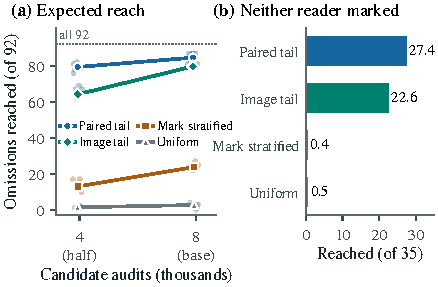
\includegraphics[width=\columnwidth]{acquisition}
\caption{\textbf{Audit reach.} (a)~Expected number of the 92 training omissions with at least one audited candidate (Eq.~\ref{eq:reach}), at the half and base budgets; faint points are the six matched draws. (b)~At half budget, expected reach among the 35 omissions on which neither weak reader placed a mark.}
\label{fig:acquisition}
\end{figure}

\begin{figure*}[t]
\centering
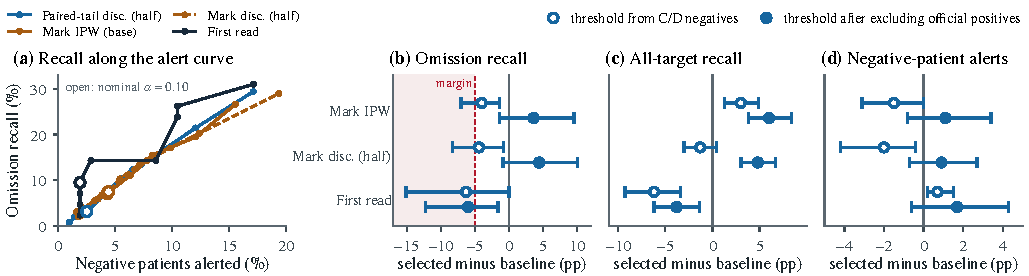
\includegraphics[width=\textwidth]{effects}
\caption{\textbf{Method comparison under two negative pools.} (a)~Mean omission recall against mean realized alerts over the calibration-derived cutoffs; open markers are the nominal $\alpha=0.10$ points of Tab.~\ref{tab:alloc}. (b--d)~Selected method minus each baseline, six-draw mean with 95\% patient-bootstrap intervals, using the same scores and the same 42 omissions, 276 targets and 90 common-negative test patients. Open circles: cutoff from C/D negatives; purple diamonds: cutoff after excluding patients with an official consensus nodule. The shaded region in (b) lies beyond the prespecified non-inferiority margin.}
\label{fig:effects}
\end{figure*}

On the 445 training patients, half-budget paired-tail sampling audits about 3,940 candidates and reaches \ReachPair{} of the 92 omissions in expectation (Fig.~\ref{fig:acquisition}a), whereas mark stratification at the base budget audits about 7,930 candidates and reaches \ReachMark{}. At the same half budget, image-tail sampling reaches \ReachImage{}, mark stratification 13.0 and uniform sampling 1.4. Most of the gain is therefore due to the image ranking, with the paired marks contributing a further 15.2 omissions on average and between 10 and 17 in each of the six matched draws. The realized draws are consistent with these expectations, ranging from 76 to 82 omissions for paired-tail sampling, 62 to 69 for image-tail sampling and 22 to 27 for base-budget mark stratification.

The improvement persists for the 35 omissions on which neither weak reader placed a mark, where the marks cannot point to the target directly (Fig.~\ref{fig:acquisition}b). Paired-tail sampling reaches 27.4 of them, compared with 22.6 for image-tail sampling and 0.4 for mark stratification at the same budget (0.9 at the base budget). In this case the marks act indirectly, by changing how the budget is distributed over the entire roster and thereby freeing reviews for highly ranked unmarked candidates. Since both paired-tail sampling and mark stratification touch nearly all 445 patients, the gain stems from which candidates are reviewed within each scan rather than from opening more scans.

\subsection{Effect of the representation}

With full reference labels, 3D features recover \OriginalLearned{} of the 276 test targets, compared with \OriginalDescriptor{} for the hand-crafted descriptors, a paired gain of 9.8 points [3.6, 16.6], while negative-patient alerts fall from 12 to 2 of 105. The fraction of covered targets that outrank every non-target candidate in their scan rises from 33.6\% to 67.9\%. As both heads share the same candidate locations, this comparison isolates the representation, and we use the 3D features in all remaining experiments.

\subsection{Main results}
\label{sec:locked}

\begin{figure*}[t]
\centering
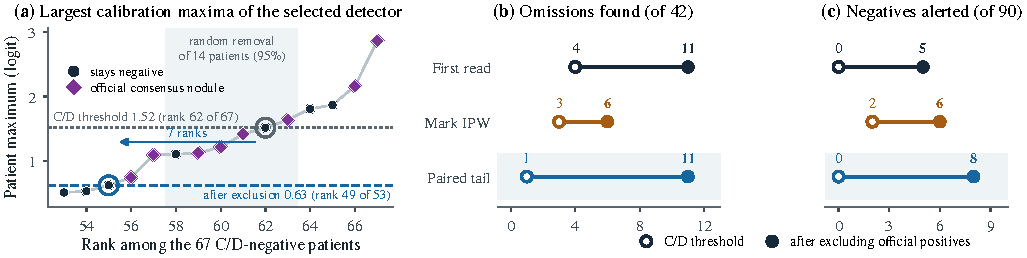
\includegraphics[width=\textwidth]{reference_tail}
\caption{\textbf{Threshold displacement at fixed scores.} (a)~The 15 largest maxima of the 67 C/D-negative calibration patients for the selected detector. Purple diamonds have a nodule in the official LUNA16 consensus. Excluding the 14 such patients moves the cutoff from rank 62 to the score at rank 55, while removing 14 patients at random puts it within the shaded ranks 58--63 (central 95\%). (b)~Omissions found among the same 42 targets, and (c)~alerts among the same 90 common-negative test patients, under the two cutoffs.}
\label{fig:tail}
\end{figure*}

\begin{table}[t]
\centering
\small
\setlength{\tabcolsep}{3.4pt}
\caption{\textbf{Locked results under the C/D reference} at nominal $\alpha=0.10$, mean of six matched draws. Omit.: recall on 42 test omissions (\%); All: recall on 276 targets (\%); Alert: negative patients alerted (\%). Half and base are audit budgets; disc.: discriminative augmentation (Eq.~\ref{eq:augmentation}). The selected method is in bold.}
\label{tab:alloc}
\begin{tabular}{lrrrr}
\toprule
Method & Omit.\,$\uparrow$ & All\,$\uparrow$ & Alert & FP/scan\,$\downarrow$ \\
\midrule
First read & \textbf{9.5} & \textbf{29.3} & 1.9 & 0.22 \\
nnPU (base) & 7.1 & 22.6 & 1.9 & 0.20 \\
Mark IPW (base) & 7.1 & 20.1 & 4.3 & 0.16 \\
Mark disc. (half) & 7.5 & 24.5 & 4.4 & 0.16 \\
Uniform disc. (half) & 7.9 & 24.9 & 5.9 & 0.16 \\
Image-tail disc. (half) & 4.8 & 23.2 & 2.4 & 0.17 \\
Paired-tail disc. (half)$^\dagger$ & 3.2 & 23.1 & 2.5 & 0.15 \\
Paired-tail IPW (half) & 4.0 & 24.9 & 2.5 & 0.15 \\
Paired-tail weighted (half) & 2.8 & 26.0 & 2.7 & \textbf{0.14} \\
\bottomrule
\end{tabular}

\end{table}

Table~\ref{tab:alloc} reports all training methods. Compared with base-budget mark IPW, the selected method uses \AuditSave\% fewer audits and raises all-target recall from 20.1\% to 23.1\%, a paired gain of 3.0 points [1.3, 4.9], at a lower alert rate (2.5\% vs.\ 4.3\%) and a similar FP/scan (0.15 vs.\ 0.16). On the primary endpoint, however, the selected method falls short. Its omission recall is \PairPrimary\%, against \IpwPrimary\% for mark IPW, a difference of $-4.0$ points [$-7.0$, $-1.4$] whose lower limit lies below the $-5$-point margin (Fig.~\ref{fig:effects}b, open circles). The conclusion is unchanged at matched alert rates: selecting each method's threshold on one calibration subset so that their alert rates on the other subset agree yields a difference of $-3.6$ points [$-7.0$, $-0.9$].

First-read training, which uses reader A's marks directly, achieves an omission recall of 9.5\%, and the half-budget mark, uniform and image-tail controls with the same estimator reach 7.5\%, 7.9\% and 4.8\%. Along the full alert curve (Fig.~\ref{fig:effects}a), first-read training leads below an alert rate of 3\%, while the audited methods remain close to one another at every rate. Results for a controlled setting in which the first reader keeps only its largest mark per scan, creating 151 imposed test omissions, are reported in the supplement.

\subsection{Analysis of missed omissions}
\label{sec:misses}

\begin{figure*}[t]
\centering
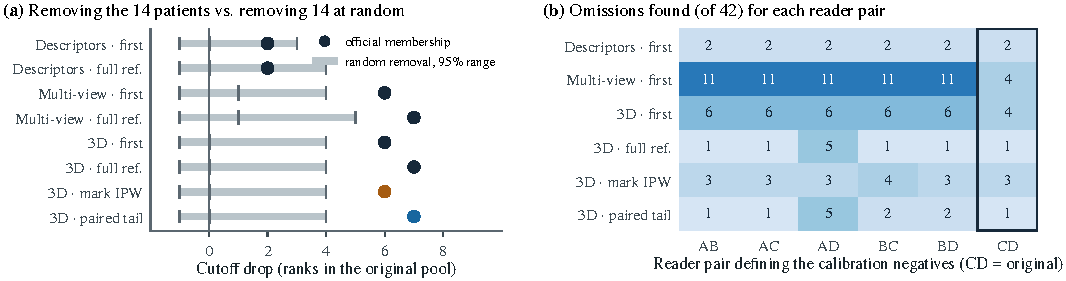
\includegraphics[width=\textwidth]{robustness}
\caption{\textbf{Robustness of the threshold displacement.} (a)~Cutoff drop on the original rank scale after excluding official-positive patients (dots), against the central 95\% range (bar, with median tick) of 8,192 subset-matched random removals. (b)~Omissions found among the same 42 targets after calibrating on the negatives of each reader pair; the boxed column is the original C/D reference.}
\label{fig:robust}
\end{figure*}

Every one of the 42 test omissions is covered by at least one candidate, so the roster itself is not the bottleneck. For the selected detector at the anchor draw, 16 omissions outrank every non-target candidate in their scan, yet only one of them exceeds the threshold. Of the 41 missed omissions, 26 are outranked by a non-target candidate in the same scan, whereas the remaining 15 win this within-scan comparison but stay below the threshold by a median of 2.22 logits. For the latter group, the failure occurs at the threshold rather than in the ranking.

The candidates that determine the threshold are unusual. Among the 45,541 candidates on C/D-negative calibration scans, only 74 lie near a contour drawn by just one of the reference readers C and D. Nevertheless, all three sampled maxima around the threshold carry this flag, as do both maxima that trigger alerts on C/D-negative test patients, and both of the latter match official LUNA16 targets. This concentration motivates the analysis of the negative pool in the next section.

\section{Effect of the Calibration Reference}
\label{sec:tail}

\subsection{Threshold displacement}

Excluding scans with an official consensus nodule removes 14 of the \PCal{} negative calibration patients and leaves \UCal{}. Three of the six largest maxima of the selected detector belong to excluded patients, and each of them matches an official nodule in 3D (Fig.~\ref{fig:tail}a). The original threshold is the 62nd score, a logit of \PairCutoffP{}, whereas the new threshold is the 49th of 53 scores, a logit of \PairCutoffU{} that ranked 55th in the original pool, a drop of \PairDrop{} ranks. Removing 14 patients at random, with the same number per calibration subset, moves the threshold by a median of \PairRobustMedian{} ranks and by at most \PairControlHi{} ranks in 95\% of the draws. The displacement is therefore driven by which patients are removed, not by the reduced pool size.

At the lower threshold, the same scores recover \PairHitsU{} of the 42 omissions instead of \PairHitsP{} (Fig.~\ref{fig:tail}b), and five of the ten additional detections were already ranked above every non-target candidate in their scan. Alerts on the same \UTest{} test patients increase from \PairAlertsP{} to \PairAlertsU{} (Fig.~\ref{fig:tail}c), which is consistent with the nominal rate of 10\%.

\subsection{Robustness}

We repeated the replay for all \NHeadRows{} fitted configurations, which yield \NHeads{} distinct score vectors over hand-crafted, multi-view and 3D features. The threshold falls for \LowerHeads{} of them, by a median of \MedianDrop{} ranks, and for \PastBand{} the drop exceeds the 95\% range of random removal. Since these score vectors share patients and include correlated training variants, the count indicates the breadth of the effect rather than independent replications.

Fig.~\ref{fig:robust}a and Tab.~\ref{tab:reference} detail eight representative detectors. The thresholds of the descriptor heads move by two ranks, within the random range, and both heads retain their two omission detections. In contrast, every learned head moves by six or seven ranks, outside the random range. A lower threshold produces additional detections only when the representation places targets between the two thresholds: the 3D first-read and full-reference heads gain 7 and 9 omissions, respectively, but the mark IPW head gains only 3. Changing the reader pair that defines the negatives yields between one and five detections for the selected detector, with at most one alert among the \RoleTest{} patients that are negative under every pair and under the official list (Fig.~\ref{fig:robust}b). The multi-view and 3D first-read heads detect 11 and 6 omissions, respectively, with every pair except the original C/D.

\begin{table}[t]
\centering\small
\setlength{\tabcolsep}{3pt}
\caption{\textbf{Fixed scores under two negative pools.} Each cell gives the count under the C/D cutoff $\to$ the count after excluding official-positive patients. Omit.: of 42 omissions; All: of 276 targets; Alert: of 90 common-negative test patients. Drop: cutoff drop in ranks of the original pool.}
\label{tab:reference}
\begin{tabular}{lrrrr}
\toprule
Scorer / training & Omit. & All & Alert & Drop \\
\midrule
Descriptors / first & 2 $\to$ 2 & 39 $\to$ 55 & 7 $\to$ 12 & 2 \\
Descriptors / full ref. & 2 $\to$ 2 & 47 $\to$ 57 & 7 $\to$ 10 & 2 \\
Multi-view / first & 4 $\to$ 11 & 66 $\to$ 125 & 1 $\to$ 7 & 6 \\
Multi-view / full ref. & 3 $\to$ 11 & 69 $\to$ 142 & 1 $\to$ 9 & 7 \\
3D / first & 4 $\to$ 11 & 81 $\to$ 133 & 0 $\to$ 5 & 6 \\
3D / full ref. & 1 $\to$ 10 & 74 $\to$ 140 & 0 $\to$ 8 & 7 \\
3D / mark IPW & 3 $\to$ 6 & 70 $\to$ 91 & 2 $\to$ 6 & 6 \\
3D / paired tail & 1 $\to$ 11 & 69 $\to$ 138 & 0 $\to$ 8 & 7 \\
\bottomrule
\end{tabular}

\end{table}

\subsection{Effect on the method comparison}

Averaged over the six matched draws, excluding official positives raises the omission recall of the selected method by \PairChange{} points \PairChangeCI{}. Its difference to mark IPW moves from $\PairRelativeP$ to $+\PairRelativeU$ points \PairRelativeUCI{}, a shift of \ReferenceInteraction{} points \ReferenceInteractionCI{} (Fig.~\ref{fig:effects}b). The same reversal occurs against mark stratification with the same estimator ($-4.4$ to $+4.4$ points), whereas the gap to first-read training remains negative. The gains in all-target recall increase under the new pool (Fig.~\ref{fig:effects}c), and the alert differences stay within about two points (Fig.~\ref{fig:effects}d), with realized alert rates of 7.2\% for paired-tail sampling and 6.1\% for mark IPW. The primary conclusion of Sec.~\ref{sec:locked} thus hinges on how the negative pool is defined rather than on the scores themselves.

\begin{figure}[t]
\centering
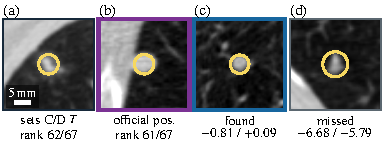
\includegraphics[width=\columnwidth]{ct_evidence}
\caption{\textbf{CT examples} (axial, 28\,mm field of view; circle: matching radius). (a)~The candidate that sets the C/D cutoff. (b)~A neighbouring calibration maximum on a scan with an official consensus nodule (purple frame). (c)~A test omission found only under the lower cutoff (blue frame). (d)~An omission below both cutoffs, outscored by a non-target candidate in its scan. Margins: best target logit minus the C/D and the new cutoff.}
\label{fig:ct}
\end{figure}

\paragraph{Qualitative examples.}
Fig.~\ref{fig:ct} relates these ranks to images. A consensus-positive maximum, shown in (b), leaves the negative pool with its score unchanged. A test omission, shown in (c), then exceeds the lower threshold with the same image, location and score. Other omissions, such as (d), remain far below both thresholds, which illustrates why ranking and calibration need to be assessed separately.
